\documentclass[a4paper, 14pt]{extarticle}
\usepackage[settings]{markdown}
\usepackage{minted}

% Поля
%--------------------------------------
\usepackage{geometry}
\geometry{a4paper,tmargin=2cm,bmargin=2cm,lmargin=3cm,rmargin=1cm}
%--------------------------------------


%Russian-specific packages
%--------------------------------------
\usepackage[T2A]{fontenc}
\usepackage[utf8]{inputenc} 
\usepackage[english, main=russian]{babel}
%--------------------------------------

\usepackage{textcomp}

% Красная строка
%--------------------------------------
\usepackage{indentfirst}               
%--------------------------------------             


%Graphics
%--------------------------------------
\usepackage{graphicx}
\graphicspath{ {./images/} }
\usepackage{wrapfig}
%--------------------------------------

% Полуторный интервал
%--------------------------------------
\linespread{1.3}                    
%--------------------------------------

%Выравнивание и переносы
%--------------------------------------
% Избавляемся от переполнений
\sloppy
% Запрещаем разрыв страницы после первой строки абзаца
\clubpenalty=10000
% Запрещаем разрыв страницы после последней строки абзаца
\widowpenalty=10000
%--------------------------------------

%Списки
\usepackage{enumitem}

%Подписи
\usepackage{caption} 

%Гиперссылки
\usepackage{hyperref}

\hypersetup {
	unicode=true
}

%Рисунки
%--------------------------------------
\DeclareCaptionLabelSeparator*{emdash}{~--- }
\captionsetup[figure]{labelsep=emdash,font=onehalfspacing,position=bottom}
%--------------------------------------

\usepackage{tempora}
\usepackage{amsmath}
\usepackage{color}
\usepackage{listings}
\lstset{
  belowcaptionskip=1\baselineskip,
  breaklines=true,
  frame=L,
  xleftmargin=\parindent,
  language=Python,
  showstringspaces=false,
  basicstyle=\footnotesize\ttfamily,
  keywordstyle=\bfseries\color{blue},
  commentstyle=\itshape\color{purple},
  identifierstyle=\color{black},
  stringstyle=\color{red},
}

%--------------------------------------
%			НАЧАЛО ДОКУМЕНТА
%--------------------------------------

\begin{document}

%--------------------------------------
%			ТИТУЛЬНЫЙ ЛИСТ
%--------------------------------------
\begin{titlepage}
\thispagestyle{empty}
\newpage


%Шапка титульного листа
%--------------------------------------
\vspace*{-60pt}
\hspace{-65pt}
\begin{minipage}{0.3\textwidth}
\hspace*{-20pt}\centering

\includegraphics[width=\textwidth]{emblem}
\end{minipage}
\begin{minipage}{0.67\textwidth}\small \textbf{
\vspace*{-0.7ex}
\hspace*{-6pt}\centerline{Министерство науки и высшего образования Российской Федерации}
\vspace*{-0.7ex}
\centerline{Федеральное государственное бюджетное образовательное учреждение }
\vspace*{-0.7ex}
\centerline{высшего образования}
\vspace*{-0.7ex}
\centerline{<<Московский государственный технический университет}
\vspace*{-0.7ex}
\centerline{имени Н.Э. Баумана}
\vspace*{-0.7ex}
\centerline{(национальный исследовательский университет)>>}
\vspace*{-0.7ex}
\centerline{(МГТУ им. Н.Э. Баумана)}}
\end{minipage}
%--------------------------------------

%Полосы
%--------------------------------------
\vspace{-25pt}
\hspace{-35pt}\rule{\textwidth}{2.3pt}

\vspace*{-20.3pt}
\hspace{-35pt}\rule{\textwidth}{0.4pt}
%--------------------------------------

\vspace{1.5ex}
\hspace{-35pt} \noindent \small ФАКУЛЬТЕТ\hspace{50pt} <<Информатика и системы управления>>

\vspace*{-16pt}
\hspace{47pt}\rule{0.83\textwidth}{0.4pt}

\vspace{0.5ex}
\hspace{-35pt} \noindent \small КАФЕДРА\hspace{50pt} <<Теоретическая информатика и компьютерные технологии>>

\vspace*{-16pt}
\hspace{30pt}\rule{0.866\textwidth}{0.4pt}
  
\vspace{11em}

\begin{center}
\Large {\bf Лабораторная работа № 2} \\ 
\large {\bf по курсу <<Базы данных>>}\\
\end{center}\normalsize

\vspace{8em}


\begin{flushright}
  {Студент группы ИУ9-51Б Горбунов А. Д.\hspace*{15pt} \\
  \vspace{2ex}
  Преподаватель Вишняков И. Э.\hspace*{15pt}}
\end{flushright}

\bigskip

\vfill
 

\begin{center}
\textsl{Москва 2024}
\end{center}
\end{titlepage}
%--------------------------------------
%		КОНЕЦ ТИТУЛЬНОГО ЛИСТА
%--------------------------------------

\renewcommand{\ttdefault}{pcr}

\setlength{\tabcolsep}{3pt}
\newpage
\setcounter{page}{2}

\section{Задача}\label{Sect::task}
\par

\begin{enumerate}
    \item Создать модель семантических объектов для предметной области, выбранной в лабораторной работе №1;
    \item Обосновать выбор кардинальных чисел атрибутов и типов объектов.
\end{enumerate}

\par

\subsection{Описание модели семантических объектов}\label{Sect::task}
Для построения модели семантических объектов было выделено три семантических объекта:

\begin{enumerate}
    \item \textbf{Student} -- сложный объект, так как имеет два объектных атрибута (\texttt{Course(Exam)}, \texttt{Course}).
    \begin{itemize}
        \item \textbf{Идентификатор:} \texttt{report\_card}. 
        Номер зачётки выбран в качестве идентификатора, так как является уникальным для каждого студента и позволяет однозначно его идентифицировать.
        \item \texttt{first\_name} – простой обязательный атрибут. Каждый студент должен иметь имя, поэтому кардинальные числа равны \texttt{1.1}.
        \item \texttt{last\_name} – простой обязательный атрибут. Так как наличие фамилии является обязательным, кардинальные числа равны \texttt{1.1}.
        \item \texttt{date\_of\_birth} – простой обязательный атрибут. Поскольку дата рождения является обязательным, кардинальные числа равны \texttt{1.1}.
        \item \texttt{encament\_date} – простой обязательный атрибут. Так как дата поступления является обязательным, кардинальные числа равны \texttt{1.1}.
        \item \texttt{email} – простой обязательный атрибут. Email является обязательным, поэтому кардинальные числа равны \texttt{1.1}.
        \item \textbf{Course(Exam)} – объектный необязательный атрибут. Экзамен является обязательным так как если у студента нет курса, то и экзамена нет, но если курс у студента есть экзаменов может быть много, поэтому кардинальные числа равны \texttt{0.N}.
        \item \textbf{Course} – объектный необязательный атрибут. Курс является необязательным, так как у студента может не быть курса, но при этом курсов может быть много, поэтому кардинальные числа равны \texttt{0.N}.
    \end{itemize}

    \item \textbf{Teacher} -- сложный объект, так как имеет два объектных атрибута (  \texttt{Course(Exam)}, \texttt{Course}).
    \begin{itemize}
        \item \textbf{Идентификатор:} \texttt{SPIN\_code}. SPIN code выбран в качестве идентификатора, так как является уникальным для каждого преподавателя и позволяет однозначно его идентифицировать.
        \item \texttt{first\_name} – простой обязательный атрибут. Каждый преподаватель должен иметь имя, поэтому кардинальные числа равны \texttt{1.1}.
        \item \texttt{last\_name} – простой обязательный однозначный атрибут. Так как наличие фамилии является обязательным, кардинальные числа равны \texttt{1.1}.
        \item \texttt{department} – простой необязательный атрибут. Поскольку преподаватель может не принадлежать какой либо кафедре, а если принадлежит, то только одной, поэтому кардинальные числа равны \texttt{0.1}.
        \item \texttt{email} – простой обязательный атрибут. Email является обязательным, поэтому кардинальные числа равны \texttt{1.1}.
        \item \textbf{Course(Exam)} – объектный необязательный атрибут. Экзамен является обязательным так, так как у преподавателя нет курса, то и экзамена нет, но если курс у преподавателя есть экзаменов может быть много, поэтому кардинальные числа равны \texttt{0.N}.
        \item \textbf{Course} – объектный необязательный атрибут. Курс является необязательным, так как у преподавателя может не быть курса, а так же курсов может быть много, поэтому кардинальные числа равны \texttt{0.N}.
    \end{itemize}

    \item \textbf{Coutse} -- гибридный объект, так как имеет групповой атрибуты \texttt{IDCourse} и \texttt{Exam}, а также содержит объектные атрибуты \texttt{Student} и \texttt{Teacher}.
    \begin{itemize}
        \item \textbf{Идентификатор:} 
        \item \textbf{IDCourse} – групповой обязательный атрибут. Идентификатор обязателен, поэтому кардинальные числа равны \texttt{1.1}.
        \begin{itemize}
            \item \texttt{title\_of\_course} – является частью идентификатора из-за чего обязателен, поэтому кардинальные числа равны \texttt{1.1}.
            \item \texttt{date\_of\_course} – является частью идентификатора из-за чего обязателен, поэтому кардинальные числа равны \texttt{1.1}.
        \end{itemize}
        \item \texttt{description} – простой необязательный атрибут. У курса как может быть, и может не быть описания, поэтому кардинальные числа равны \texttt{0.1}.
        \item \texttt{department} – простой обязательный атрибут. У курса обязательно есть кафедра, которая его проводит, поэтому кардинальные числа равны \texttt{1.1}.
        \item \texttt{schedule} – простой необязательный атрибут. Поскольку расписание может отсутствовать, поэтому кардинальные числа равны \texttt{0.1}.
        \item \textbf{Exam} – групповой обязательный атрибут. У любого курса должен быть экзамен, причём их может быть несколько, поэтому кардинальные числа равны \texttt{1.N}.
        \begin{itemize}
            \item \textbf{Идентификатор:} 
            \item \textbf{IDExem} – групповой обязательный атрибут. Идентификатор обязателен, поэтому кардинальные числа равны \texttt{1.1}.
            \begin{itemize}
                \item  \texttt{time\_stamp} - является частью идентификатора, поэтому кардинальные числа равны \texttt{1.1}.
                \item \textbf{Student} – является частью идентификатора, кардинальные числа равны \texttt{1.1}.
            \end{itemize}
            \item \texttt{grade} – простой обязательный атрибут. После проведения экзамена обязательно должна быть оценка, поэтому кардинальные числа равны \texttt{1.1}.
            \item \textbf{Teacher} – объектный обязательный атрибут. Преподаватель должен принимать экзамен, для его проведения, поэтому кардинальные числа равны \texttt{1.1}.
        \end{itemize}
        \item \textbf{Theacher} – объектный необязательный атрибут. У курса как может не быть преподавателя, так и может быть несколько, поэтому кардинальные числа равны \texttt{0.N}.
        \item \textbf{Student} – объектный необязательный атрибут. У курса как может не быть студентов, так и может быть много, поэтому кардинальные числа равны \texttt{0.N}.
    \end{itemize}
\end{enumerate}

Визуализация модели семантических объектов изображена на рисунке~\ref{fig:scheme}.

\begin{figure}[!htb]
	\centering
	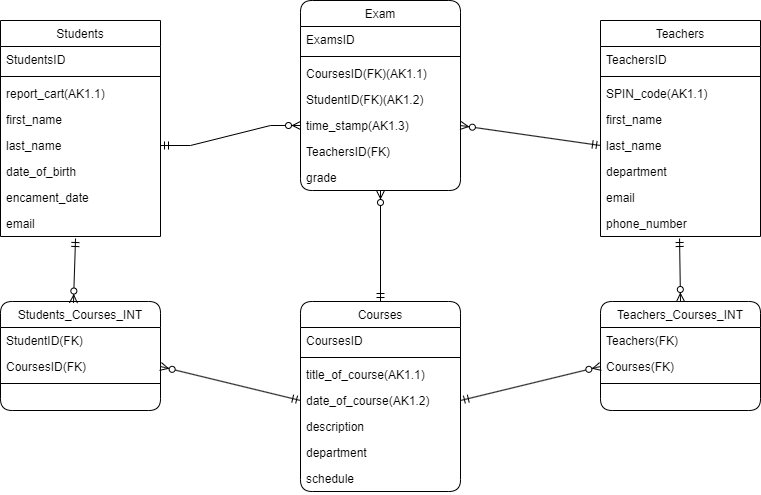
\includegraphics[width=0.8\textwidth]{scheme.png}
\caption{Модель семантических объектов}
\label{fig:scheme}

\end{figure}
\end{document}
